%!TEX root = mb.tex


\section{Introduction}\label{sec:intro}


    Network processing appliances (``middleboxes'') such as firewalls, NATs, proxies, and intrusion detection systems are crucial components of modern networks~\cite{aplomb}. 
     In recent trends, more and more organizations are {\it outsourcing} their network processing, either to cloud providers~\cite{aplomb, aryaka, zscalar} or to service providers through Network Functions Virtualization (NFV)~\cite{nfv} who now run  middleboxes for the organizations. This strategy promises to reduce costs, decrease the burden of managing and configuring these devices, and provide elasticity and fault tolerance, as documented in~\cite{aplomb}.
Already now, the NFV working group~\cite{nfvwg} has over 250 members ranging from large telecoms to hardware manufacturers, all of whom are investing in new technologies to enable outsourced traffic processing.
   
   Nevertheless, outsourcing middleboxes to a third party service provider brings a new and important challenge: the confidentiality of the traffic. In order to be able to process and examine the traffic of an organization, the cloud  receives  the traffic {\em unencrypted}.  This means that the cloud now has access to potentially sensitive packet payloads,  IP addresses, and ports revealing confidential information about the organization. This situation is worrisome considering the number of documented data breaches by cloud employees or hackers gaining access to clouds~\cite{PrivacyRecords}.
   Hence, an important question is: can we enable a third party to perform traffic processing for an enterprise, {\em without seeing the enterprise's traffic}?
   
   
   

% Justine's text unchanged: (the above is a combination of Justine & Raluca)
%    Network processing appliances (''middleboxes'') such as firewalls, proxies, and intrusion detection systems make up a substantial fraction of modern network infrastructure; studies show that as much as 1/3 of enterprise network hardware consists of such devices~\cite{aplomb}.
%    However, recent trends suggest that this fraction may begin to decline as more and more networks begin to {\it outsource} their network processing, either to cloud providers~\cite{aplomb, aryaka, zscalar} or to service providers through Network Functions Virtualization (NFV)~\cite{nfv}.
%    At the time of this writing, the NFV working group~\cite{nfvwg} has over 250 members ranging from large telecoms to hardware manufacturers, all of whom are investing in new technologies to enable outsourced traffic processing.
%    For consumers, outsourcing traffic processing offers many of the same benefits that outsourcing compute and storage have attained through cloud computing: decreased costs, ease of management, the ability to scale and failover on demand, \etc{}.
%    Nevertheless, outsourcing network processing brings new challenges, and among them, an issue which is critical to most enterprises: privacy.
%    
%    Under traditional middlebox deployments, traffic is processed and inspected by devices which are owned, hosted, and managed entirely within the enterprise itself.
%    Encrypted traffic is often decrypted to enable deep packet inspection (DPI) such as intrusion detection and exfiltration detection.
%    This configuration places critical trust in the hands of network administrators, who can potentially read or even modify {\it any} connection within the company.
%    Outsourcing shifts this trust away from network administrators who are employed and monitored by the company whose data is being processed, and to a third party company with its own employees, hiring practices, and motivations.
%    Hence, in this paper, we ask: is it possible to enable a third party to perform traffic processing for an enterprise, without transferring the ability to read and monitor the enterprise's traffic?
%    
% 
     
     
     
  
    We design and build \sys (read ``embark"), the first system that enables running a wide range of middleboxes at a cloud  while maintaining the confidentiality of the traffic. \sys provides these guarantees even against attackers who gained access to {\em all} the data at the cloud.  \sys's name concatenates the words MB (middlebox) and Ark (protection). \sys supports a wide range of middleboxes, in fact, all middleboxes that~\cite{aplomb} documents to be fit for cloud outsourcing. We list these middleboxes in Table~\ref{tab:apps-ops}. Moreover, \sys supports these middleboxes with competitive performance. 
    
    The approach in \sys is to encrypt the traffic that goes to  the middleboxes in the cloud and enables the cloud to process encrypted traffic without ever decrypting it. \sys encrypts the packet payload as well as important information in the header (such as IP addresses and ports). Since the service provider receives only encrypted traffic and no decryption key, it cannot see the confidential data. However, designing a practical system that supports a wide-range of middlebox applications over encrypted traffic is challenging and required a set of new cryptographic and systems techniques.
    
    
\newcounter{theapp} \setcounter{theapp}{0}  
\newcommand{\capp}{\refstepcounter{theapp}\arabic{theapp}}
    
\begin{table}[t!]
\centering  
\begin{tabular}{c|p{3.3cm}|p{0.6cm}|p{2.5cm}}
& {\bf Middlebox}  & {\bf Type } & {\bf Example fields}  \\
\hline \hline
\capp &  IP Firewall \S\ref{sec:firewall} & HO &  IP address   \\
\capp &  Application Firewall  \S\ref{sec:firewall} & BA & IP address  \\
\capp & NAT  \S\ref{sec:nat} & HO & IP address  \\
\capp & IP Forwarding  \S\ref{sec:other_apps}  & HO &  IP address \\
\capp & Load Balancer L4 \S\ref{sec:loadb} & HO & IP address  \\
\capp & Load Balancer L7 \S\ref{sec:loadb} & BA & URL in payload  \\
\capp & Web Proxy/Cache  \S\ref{s:proxy} & HO & URL in payload \\
\capp & Intrusion Detect (IDS) \S\ref{sec:ids} & BA & payload \\
\capp & Data Exfiltration  \S\ref{sec:ids} & BA & payload \\
\capp & VPN Gateway \S\ref{sec:vpn} &  HO &  IP address \\ 
\end{tabular}
\caption{Middleboxes supported by \sys, shown with the section that discusses them, their type, HO (header only) or BA (bytestream aware), and one  example of an encrypted field  each operates on. \label{tab:apps-ops} }
\end{table}

% 2nd fig/1st fig = 1.12 ratio
\begin{figure*}[t!]
\centering
\subfigure[Enterprise to external site communication]{
  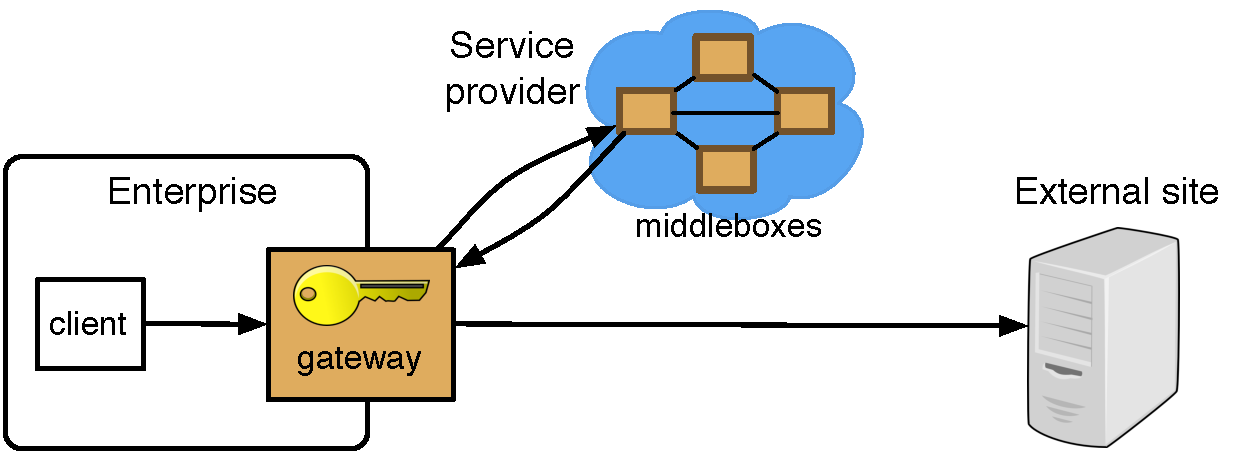
\includegraphics[width=3.0in]{fig/model_1.pdf}
  \label{fig:model1} }
%
\hfill  
\subfigure[Enterprise to enterprise communication]{
   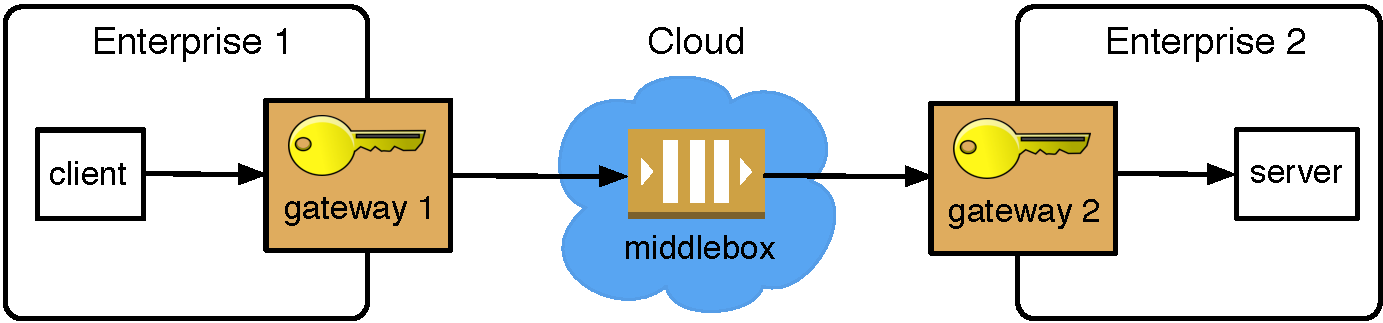
\includegraphics[width=3.6in]{fig/model_2.pdf}
     \label{fig:model2}}
     
     %
\caption{System architecture. Aplomb and NFV system setup with \sys encryption  at the gateway. The arrows indicate traffic from the client to the server; the response traffic follows the reverse direction. \label{fig:sys-overview}}
\end{figure*}


    
The first challenge is that performing generic computation on encrypted data is prohibitively practical. The applications considered provide complex functionalities. For example, firewall and NAT examine packet header information such as IP addresses and ports; for IDS and data exfiltration detection, the middlebox (MB) examines the packet payload and tries to match complex rules (e.g., keywords, regular expressions). For each packet, a middlebox must process a packet on the timescale of microseconds. Existing generic homomorphic encryption schemes are many orders of magnitude impractical~\cite{gentry:fhe-aes-eprint}, not just for middleboxes but for most systems (even those with more relaxed performance requirements).

Fortunately, recently, a recent paper, CryptDB~\cite{popa:cryptdb}, put forth a new vision for building practical such systems, and we are inspired by this vision too. Instead of using a generic encryption scheme, the idea is to identify core operations that underlie the functionality of the system and to support each with a specialized and fast encryption scheme. Unfortunately, neither the core operations nor the encryption schemes in CryptDB fit in our network setting so we need to start from zero.

We studied the relevant middleboxes, and we managed to identify two core operations that underlie all these middleboxes: {\em keyword match} and {\em range match}. Keyword match refers to  identifying if a keyword appears in a byte stream at some offset.   For example, keyword match is useful for an HTTP proxy \todo{http proxy or web proxy}: the service provider can identify if a filename cached at the proxy appears in a http GET request in the packet flow. % data exfiltration when a watermark is searched for in the traffic, for IDS when malicious strings are searched for in the traffic and for web proxy for matching file identifiers that could be potentially in a cache. 
Range match enables determining if a value $x$ is in an interval [$x_1$, $x_2$]. An example middlebox that uses range match is the firewall.   For example, the firewall has to determine if a source IP address from a packet falls in a certain range of IP addresses and, if so, apply a certain action to the packet.  Note that range match supports a basic version of keyword match, namely complete equality check, when the range consists of only one value.
%
Table~\ref{tab:apps-ops} summarizes the middleboxes we support and the operations they rely on. 


% TO CUT/REMOVE: just say that they are too insecure and slow and don't explain about order
A second challenge is that there is no suitable encryption scheme for the range match scheme:
 the only practical schemes applicable here, order-preserving encryption (OPE)~\cite{boldyreva:ope,popa:mope}, are both too insecure and too slow for our setting.  For example, OPE schemes leak the order of the values encrypted. We designed a new encryption scheme, called {\em RangeMatch}, which is targeted at and takes advantage of the network setting. RangeMatch  is fast (performing encryptions in under 3$\mu$s, 3 orders of magnitude faster than the OPE schemes) and it is more secure because it does not reveal the order of the values encrypted. 
 
A last challenge is to design and build a system that supports the variety of applications mentioned, is practical and easy to deploy. 
To address this challenge, we make the following contributions:
\begin{itemize}
\item we design a  protocol for each type of middlebox in Table~\ref{tab:apps-ops} by employing our two match  primitives,
\item  we integrate these protocols in a way that {\em does not change the existing packet structure}. We achieve this by ensuring that our encrypted values fit into the space of the unencrypted values, use the options header, and sometimes add a second network flow.
\item  for most middleboxes, we keep {\em unchanged  the algorithms employed on the fast path} which can run identically on the encrypted traffic. In particular, firewalls implemented in hardware can use the existing hardware unchanged.  This enables \sys's performance on the fast path to be fast. 
\end{itemize}




We implemented and evaluated \sys. As mentioned, we support all applications fit in the cloud outsourcing model, as surveyed in~\cite{aplomb} -- any appliance which it outsourced today can also be outsourced using \sys.
Further, \sys imposes very negligible throughput overheads at the service provider: for example, a firewall operating over encrypted data achieves \todo{XXX} where a firewall over unencrypted data achieves \todo{YYY} -- an only \todo{ZZZ}\% penalty. Our gateway can forward at 1.5 Gbps on a single core; our 8 core server can easily saturate a 10Gbps link. \todo{adjust this sentence}
